\documentclass[conference]{IEEEtran}

\usepackage{amsmath,amsfonts}
\usepackage{graphicx}
\usepackage{cite}
\usepackage{xcolor}
\usepackage{booktabs}
\usepackage{multirow}
\usepackage{array}
\usepackage{float}
\usepackage{url}
\usepackage{listings}

% Numbers below are generated by mllab5.py (run it first).
\newcommand{\nTrain}{840}
\newcommand{\nTest}{360}
\newcommand{\bestKNormal}{3}
\newcommand{\bestAccNormal}{88.61}
\newcommand{\bestKWeighted}{3}
\newcommand{\bestAccWeighted}{89.17}
\newcommand{\trainAccThree}{92.26}
\newcommand{\testAccThree}{88.61}
\newcommand{\gapAccThree}{3.65}
\newcommand{\trainAccOne}{100.00}
\newcommand{\testAccOne}{86.67}
\newcommand{\trainAccLast}{87.38}
\newcommand{\testAccLast}{87.22}
\newcommand{\lastK}{15}
\newcommand{\maxDiffAll}{0.00}


\title{k-Nearest Neighbors Classification of Uniswap V3 Swap Fee Tiers: Manual Implementation and Comparison with Scikit-learn}

\author{%
  \parbox{\textwidth}{\centering
    \fontsize{9}{10}\selectfont
    Author~One$^{1}$,\;
    Author~Two$^{1}$,\;
    Author~Three$^{1}$,\\[4pt]
    \textit{$^{1}$Department of Computer Science and Engineering,}\\
    \textit{Amrita School of Computing, Amrita Vishwa Vidyapeetham, Bengaluru, India}\\[4pt]
    \footnotesize
    email1@bl.students.amrita.edu,\;
    email2@bl.students.amrita.edu,\;
    email3@bl.students.amrita.edu,\\
  }
}

\begin{document}

\maketitle
\begin{abstract}

This laboratory exercise implements the k-Nearest Neighbors (k-NN) classifier from first principles and evaluates it on transaction data from the Uniswap V3 decentralized exchange. The classification target is the pool fee tier, restricted to two classes. The implementation is modular and covers categorical encoding, missing-value imputation, configurable distance metrics, four configurable sorting algorithms, nearest-neighbor selection with deterministic tie breaking, majority voting, and distance-weighted voting. The classifier is exposed through \texttt{fit()}, \texttt{predict()} and \texttt{score()} methods and compared with the scikit-learn \texttt{KNeighborsClassifier} for odd values of $k$ from 1 to 15, with and without distance weighting. Train and test accuracy, precision, recall and F1-score are used to discuss class separation, over-fitting and under-fitting.

\end{abstract}

\begin{IEEEkeywords}

k-Nearest Neighbors,
Classification,
Distance Weighting,
Uniswap V3,
Scikit-learn,
Python

\end{IEEEkeywords}

%%%%%%%%%%%%%%%%%%%%%%%%%%%%%%%%%%%%%%%%%%%%%%%%%%%%%%%%%%%%%%

\section{Introduction}

The k-Nearest Neighbors rule classifies a sample by the majority class among its $k$ closest training samples \cite{cover1967}. It has no training phase beyond storing the data, which makes it simple to implement and a useful baseline for studying how a classifier behaves as its single hyper-parameter, $k$, changes.

The project data set contains transaction-level records of swaps executed on Uniswap V3. Each record describes the time of the swap, the two tokens involved and their decimals, the swapped amounts and their USD value, the block number, the gas used and the gas price, together with the fee tier of the pool through which the swap was executed. Fee tiers are stored in hundredths of a basis point (for example, 100 is 0.01\% and 3000 is 0.3\%).

In this laboratory the target is \texttt{fee\_tier}, restricted to the two classes 100 and 3000, so the task is a binary classification problem: given the characteristics of a swap, predict which fee tier the swap was routed through. The target column is excluded from the input features to avoid target leakage. A balanced sample of 600 swaps per class was used, giving 1,200 observations.

%%%%%%%%%%%%%%%%%%%%%%%%%%%%%%%%%%%%%%%%%%%%%%%%%%%%%%%%%%%%%%

\section{Objectives}

\begin{itemize}

\item Design a modular k-NN classifier with encoding, imputation, distance calculation, configurable sorting, neighbor identification and class assignment.

\item Extend the classifier with distance-weighted voting.

\item Split the data into training and test sets and study the scikit-learn \texttt{KNeighborsClassifier}.

\item Provide \texttt{fit()}, \texttt{predict()} and \texttt{score()} in the developed package.

\item Compare the developed classifier with the package classifier for a range of $k$, with and without weighting.

\item Discuss class separation, over-fitting and under-fitting from the observed results.

\end{itemize}

%%%%%%%%%%%%%%%%%%%%%%%%%%%%%%%%%%%%%%%%%%%%%%%%%%%%%%%%%%%%%%

\section{Literature Survey}

% TODO: replace the placeholder rows with the papers downloaded for the project.
Table~\ref{tab:literature} summarizes the papers studied for this project.

\begin{table}[h]
\centering
\caption{Literature Survey}
\label{tab:literature}

\begin{tabular}{|p{1.4cm}|p{2.0cm}|p{3.8cm}|}

\hline

\textbf{Paper} &
\textbf{Problem / Method} &
\textbf{Finding and Relevance}

\\ \hline

\textit{Add paper 1} & \textit{...} & \textit{...} \\ \hline

\textit{Add paper 2} & \textit{...} & \textit{...} \\ \hline

\textit{Add paper 3} & \textit{...} & \textit{...} \\ \hline

\end{tabular}

\end{table}

The foundational result for the method used here is the nearest neighbor rule of Cover and Hart \cite{cover1967}, and the inverse-distance weighting implemented in this laboratory is a variant of the distance-weighted rule of Dudani \cite{dudani1976}.

%%%%%%%%%%%%%%%%%%%%%%%%%%%%%%%%%%%%%%%%%%%%%%%%%%%%%%%%%%%%%%

\section{Methodology}

\subsection{Data Preprocessing}

The raw data set was filtered to the two selected fee tiers and a balanced random sample of 600 rows per class was drawn with a fixed seed. The data was then divided into a stratified 70:30 training and test split, giving \nTrain{} training and \nTest{} test samples. Every statistic below was learned from the training part only and then applied to the test part.

\begin{itemize}

\item \textbf{Imputation:} missing numeric values are replaced by the training median and missing categorical values by the training mode.

\item \textbf{Encoding:} the token symbols are converted to numbers by frequency encoding; a category not seen in training is encoded as zero.

\item \textbf{Transformation:} the heavy-tailed fields (the two token amounts, the USD amount, gas used and gas price) are compressed using $\operatorname{sign}(x)\log(1+|x|)$.

\item \textbf{Standardization:} every feature is scaled to zero mean and unit variance.

\end{itemize}

\subsection{A1 -- Modular k-NN}

The classifier is built from independent functions for distance calculation, sorting, neighbor identification and voting. The distance between a query $x$ and a training sample $x_i$ can be computed with the Euclidean, Manhattan or Chebyshev metric; the Euclidean distance is

\begin{equation}
d(x,x_i)=\sqrt{\sum_{j}(x_j-x_{ij})^2}.
\end{equation}

The training samples are sorted by distance using one of four algorithms selected through a configuration parameter: bubble sort, insertion sort, selection sort and merge sort. The quadratic algorithms have $O(n^2)$ cost per query, while merge sort has $O(n\log n)$ cost and is used for the experiments over the complete data set.

Every sorted entry is stored as (distance, training index, label). When two samples are at equal distance, the one with the smaller training index is placed first, which gives a deterministic neighbor order. The $k$ nearest neighbors are the first $k$ entries, and the class is assigned by majority vote. If two classes receive the same number of votes, the smaller class label is chosen.

\subsection{A2 -- Weighted k-NN}

In the weighted version a neighbor at distance $d_i$ contributes the weight

\begin{equation}
w_i=\frac{1}{\max(d_i,\epsilon)},
\end{equation}

where a very small $\epsilon$ prevents division by zero when a neighbor coincides with the query. The predicted class is the one with the largest total weight, and an exact tie again goes to the smaller label. This is an inverse-distance variant of the distance-weighted rule introduced by Dudani \cite{dudani1976}.

\subsection{A3 to A7 -- Split, scikit-learn and the \texttt{fit/predict/score} Interface}

The train and test sets are produced with \texttt{train\_test\_split} using \texttt{test\_size=0.3} and stratification, so both classes remain balanced. A scikit-learn \texttt{KNeighborsClassifier} \cite{sklearn} with $k=3$ is trained on the training set (A4), its accuracy is measured with \texttt{score()} (A5) and its behavior on the test vectors is studied with \texttt{predict()} (A6). The developed functions are packaged into the class \texttt{ManualKNN} with the methods \texttt{fit()}, \texttt{predict()} and \texttt{score()} (A7).

\subsection{A8 and A9 -- Comparison for Different $k$}

The developed classifier and the scikit-learn classifier are evaluated on the same train and test data for $k=1,3,5,\dots,15$. The experiment is repeated with distance weighting, using \texttt{weights='distance'} for scikit-learn. Training accuracy of the package classifier is also recorded for every $k$ to study the fit of the model.

\subsection{Software Quality}

All functionality is implemented as functions inside a single module, print statements appear only in the main program, and the code was verified with unit tests written using the \texttt{unittest} framework \cite{unittest}. The tests cover preprocessing, the four sorting algorithms, distance metrics, tie breaking, voting, agreement with scikit-learn, and invalid parameters. Numerical computation uses NumPy \cite{numpy} and pandas \cite{pandas}.

%%%%%%%%%%%%%%%%%%%%%%%%%%%%%%%%%%%%%%%%%%%%%%%%%%%%%%%%%%%%%%

\section{Experimental Results}

\subsection{A5 -- Scikit-learn Accuracy for $k=3$}

For $k=3$ the training accuracy was \trainAccThree\% and the test accuracy was \testAccThree\%. Table~\ref{tab:metrics} lists the per-class precision, recall and F1-score on the test set.

\begin{table}[h]
\centering
\caption{Per-Class Test Metrics for $k=3$}
\label{tab:metrics}

\begin{tabular}{|c|c|c|c|c|}

\hline

\textbf{Class} & \textbf{Precision} & \textbf{Recall} & \textbf{F1} & \textbf{Support}

\\ \hline

100 & 0.8757 & 0.9000 & 0.8877 & 180 \\ \hline
3000 & 0.8971 & 0.8722 & 0.8845 & 180 \\ \hline


\end{tabular}

\end{table}

\subsection{A8 -- Manual versus Scikit-learn k-NN}

Table~\ref{tab:a8} reports the test accuracy of the developed and the scikit-learn classifier, together with the scikit-learn training accuracy, for every tested value of $k$.

\begin{table}[h]
\centering
\caption{Accuracy of k-NN for Different Values of $k$}
\label{tab:a8}

\begin{tabular}{|c|c|c|c|}

\hline

\textbf{$k$} & \textbf{Manual Test} & \textbf{Sklearn Test} & \textbf{Sklearn Train}

\\ \hline

1 & 86.67\% & 86.67\% & 100.00\% \\ \hline
3 & 88.61\% & 88.61\% & 92.26\% \\ \hline
5 & 88.06\% & 88.06\% & 91.55\% \\ \hline
7 & 86.67\% & 86.67\% & 89.76\% \\ \hline
9 & 86.67\% & 86.67\% & 88.93\% \\ \hline
11 & 86.39\% & 86.39\% & 89.17\% \\ \hline
13 & 86.39\% & 86.39\% & 88.45\% \\ \hline
15 & 87.22\% & 87.22\% & 87.38\% \\ \hline


\end{tabular}

\end{table}

Figure~\ref{fig:a8} shows the comparison and Figure~\ref{fig:fit} shows how the training and test accuracy change with $k$.

\begin{figure}[h]

\centering

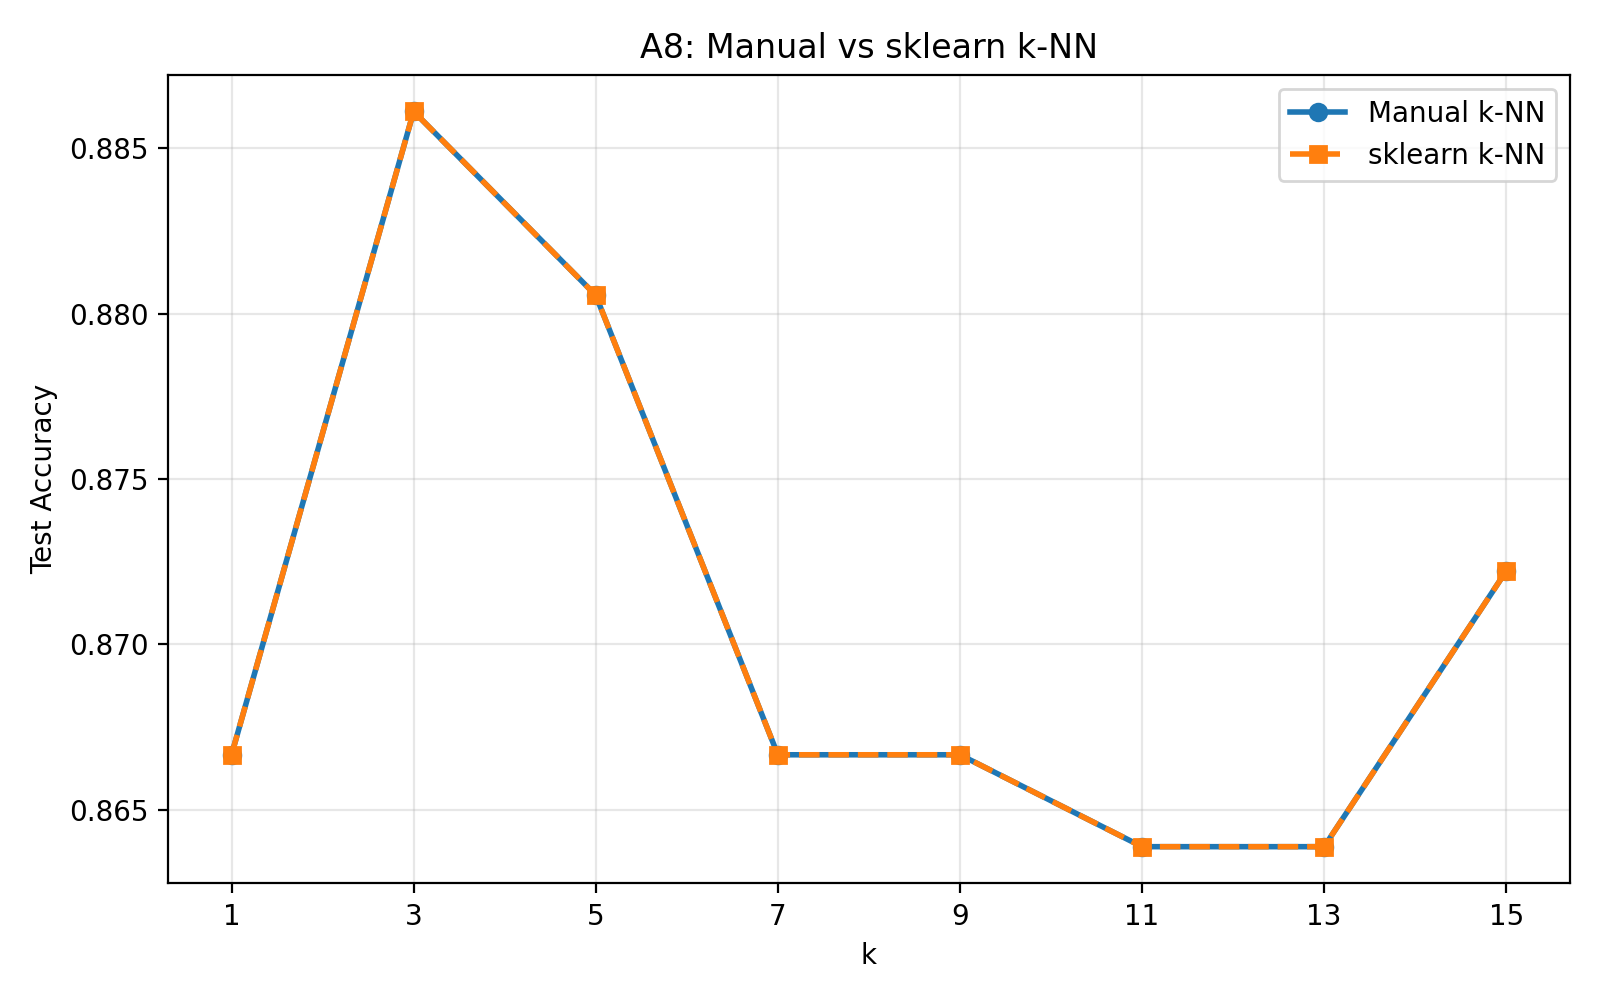
\includegraphics[width=\columnwidth]{figures/A8_accuracy_comparison.png}

\caption{Manual versus scikit-learn k-NN test accuracy}

\label{fig:a8}

\end{figure}

\begin{figure}[h]

\centering

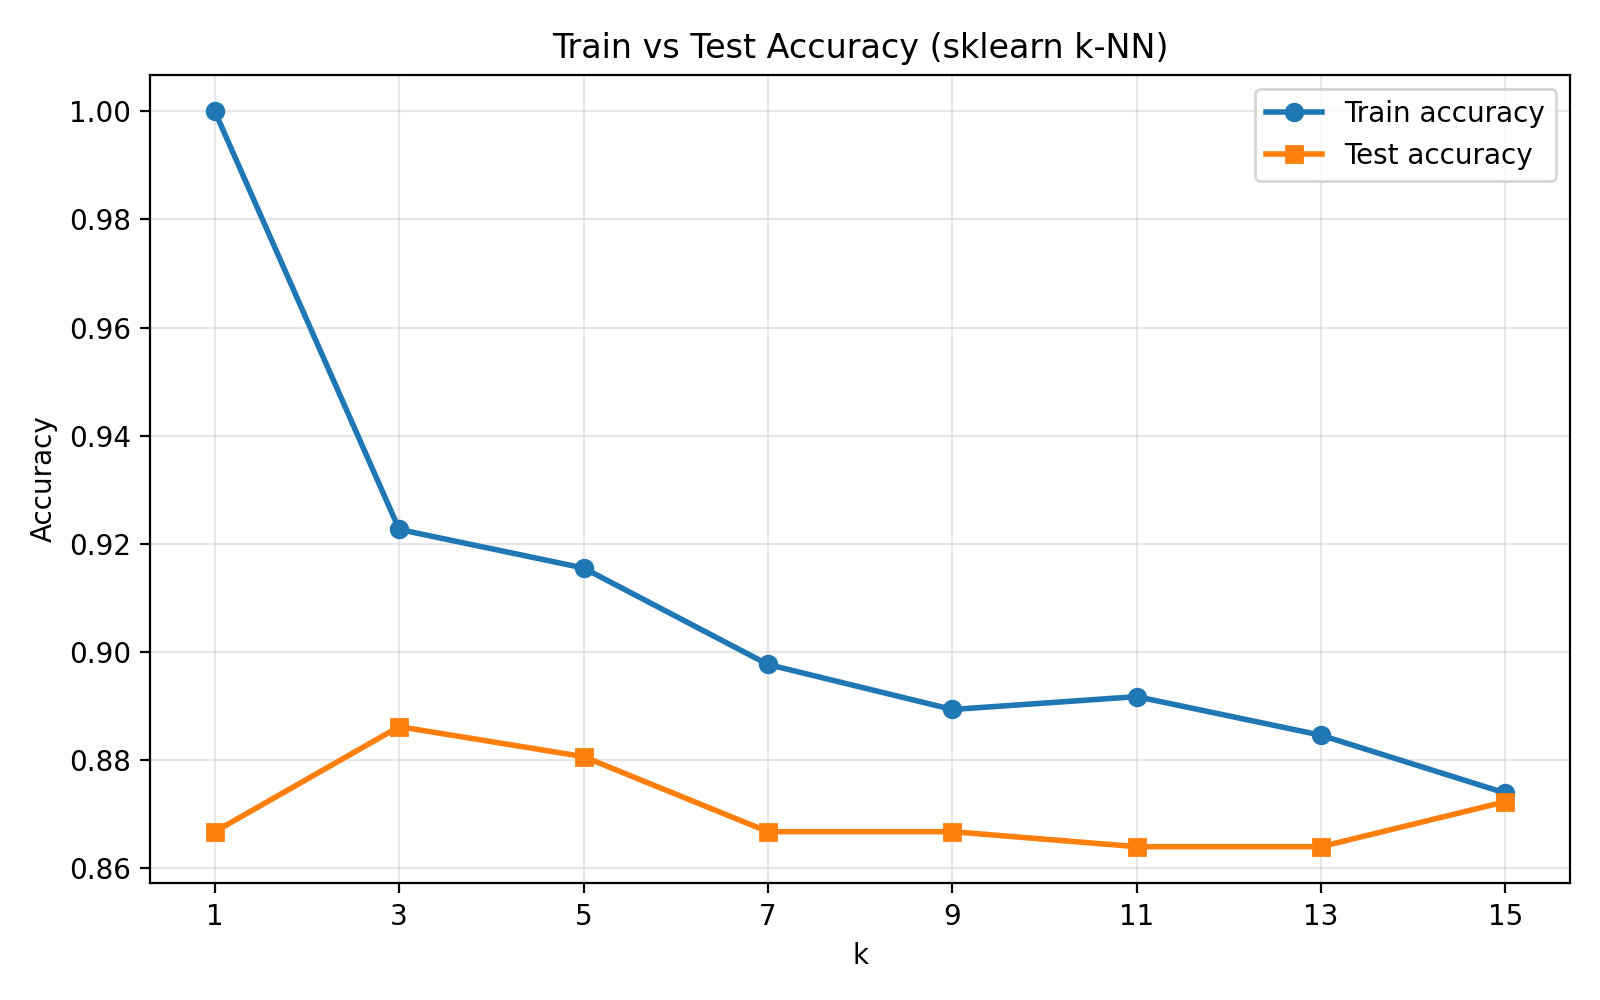
\includegraphics[width=\columnwidth]{figures/train_test_accuracy.png}

\caption{Training and test accuracy of k-NN against $k$}

\label{fig:fit}

\end{figure}

\subsection{A9 -- Weighted k-NN}

Table~\ref{tab:a9} and Figure~\ref{fig:a9} report the weighted experiment. The best weighted test accuracy was \bestAccWeighted\% at $k=\bestKWeighted$, compared with \bestAccNormal\% at $k=\bestKNormal$ for the unweighted classifier.

\begin{table}[h]
\centering
\caption{Test Accuracy of Weighted k-NN}
\label{tab:a9}

\begin{tabular}{|c|c|c|}

\hline

\textbf{$k$} & \textbf{Manual Weighted} & \textbf{Sklearn Weighted}

\\ \hline

1 & 86.67\% & 86.67\% \\ \hline
3 & 89.17\% & 89.17\% \\ \hline
5 & 89.17\% & 89.17\% \\ \hline
7 & 87.50\% & 87.50\% \\ \hline
9 & 88.06\% & 88.06\% \\ \hline
11 & 86.94\% & 86.94\% \\ \hline
13 & 87.50\% & 87.50\% \\ \hline
15 & 88.33\% & 88.33\% \\ \hline


\end{tabular}

\end{table}

\begin{figure}[h]

\centering

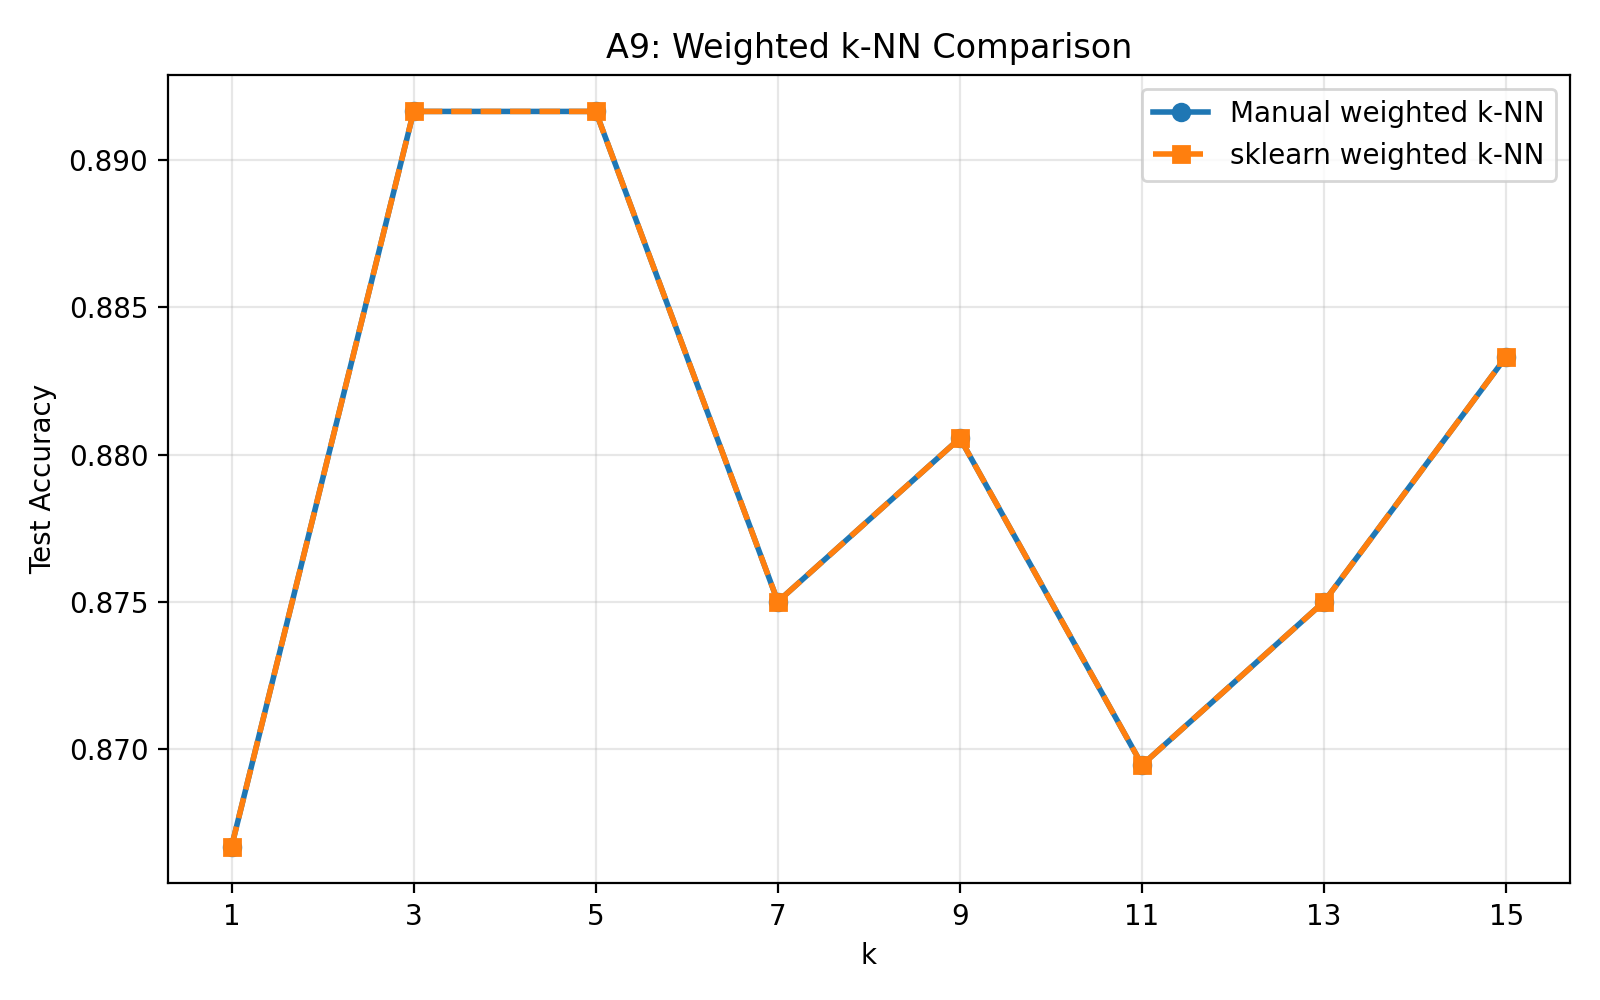
\includegraphics[width=\columnwidth]{figures/A9_weighted_comparison.png}

\caption{Weighted k-NN comparison for different values of $k$}

\label{fig:a9}

\end{figure}

%%%%%%%%%%%%%%%%%%%%%%%%%%%%%%%%%%%%%%%%%%%%%%%%%%%%%%%%%%%%%%

\section{Discussion}

% NOTE: re-read each paragraph after running mllab5.py on the real data.
% The numbers are filled in automatically, but the wording must match them.

\subsection{Are the Classes Well Separated?}

The highest test accuracy was \bestAccNormal\%, which is far above the 50\% expected from guessing on a balanced test set, so the selected features carry real information about the fee tier. The accuracy is, however, clearly below 100\%, and Table~\ref{tab:metrics} shows that errors occur in both classes. The two classes are therefore separable to a useful degree but they overlap in feature space, so some swaps have neighbors from both fee tiers.

\subsection{Effect of Increasing $k$}

For $k=1$ the prediction depends on a single training sample, so the decision boundary follows individual points, including noisy ones. As $k$ grows, more neighbors vote and the boundary becomes smoother. In Table~\ref{tab:a8} the test accuracy changes from \testAccOne\% at $k=1$ to \testAccLast\% at $k=\lastK$, with the best value, \bestAccNormal\%, at $k=\bestKNormal$.

\textit{Over-fitting} occurs when $k$ is too small: the model memorizes the training set, so the training accuracy is very high (\trainAccOne\% at $k=1$) while the test accuracy is lower (\testAccOne\%). \textit{Under-fitting} occurs when $k$ is too large: the neighborhood covers a large part of the training set and the vote approaches the overall class proportions, so local structure is lost and both training and test accuracy fall. For a balanced two-class problem the extreme case $k=n$ would predict the same class for every sample.

\subsection{Is k-NN a Good Classifier for this Data?}

The classes are balanced, so accuracy is a meaningful measure, and precision, recall and F1-score in Table~\ref{tab:metrics} are of similar size for both classes, which shows that the classifier is not favoring one fee tier. Based on these metrics, k-NN with a suitable $k$ is a reasonable classifier for this data set. Its main drawbacks are that every prediction requires distances to all training samples and that it is sensitive to feature scaling, which is why standardization is applied.

\subsection{Does the Model Show a Regular Fit?}

For $k=3$ the training accuracy is \trainAccThree\% and the test accuracy is \testAccThree\%, a gap of \gapAccThree{} percentage points. Training accuracy is high, so the model is not under-fitting. A moderate gap indicates some variance: the model does better on samples it has stored than on unseen ones. Figure~\ref{fig:fit} shows that the gap is largest for the smallest $k$ and narrows as $k$ increases (from \trainAccOne\% against \testAccOne\% at $k=1$ to \trainAccLast\% against \testAccLast\% at $k=\lastK$), so a moderate $k$ gives a more regular fit than $k=1$.

\subsection{When Does Over-fitting Occur?}

Over-fitting occurs for very small $k$, most clearly $k=1$, where every training sample is its own nearest neighbor and the training accuracy reaches \trainAccOne\%. With distance weighting a training sample at distance zero receives the whole vote, so the training accuracy of the weighted classifier is essentially 100\% for every $k$ and cannot be used to judge fit; only the test accuracy is informative there.

\subsection{Effect of Distance Weighting}

Table~\ref{tab:a9} should be compared with Table~\ref{tab:a8}. Weighting gives closer neighbors more influence and mainly matters when the $k$ neighbors contain both classes and the nearest ones belong to one class. The best weighted accuracy was \bestAccWeighted\% at $k=\bestKWeighted$, against \bestAccNormal\% for the unweighted classifier. Over all tested values of $k$ in both experiments, the largest difference between the test accuracy of the developed classifier and that of scikit-learn was \maxDiffAll{} percentage points, which checks the distance calculation, sorting, neighbor selection and voting against the package.

%%%%%%%%%%%%%%%%%%%%%%%%%%%%%%%%%%%%%%%%%%%%%%%%%%%%%%%%%%%%%%

\section{Conclusion}

A modular k-NN classifier was implemented for a binary classification problem built from Uniswap V3 swap data. It supports several distance metrics, four configurable sorting algorithms, deterministic tie breaking, majority and distance-weighted voting, and a \texttt{fit/predict/score} interface. For $k=3$ the test accuracy was \testAccThree\%; over all tested values the best unweighted test accuracy was \bestAccNormal\% at $k=\bestKNormal$ and the best weighted accuracy was \bestAccWeighted\% at $k=\bestKWeighted$.

The experiments show how the choice of $k$ balances sensitivity to individual samples (small $k$, high training accuracy and a larger gap to the test accuracy) against smoothing (larger $k$). The largest difference between the developed classifier and scikit-learn was \maxDiffAll{} percentage points in test accuracy, and the unit tests verify the individual components.

%%%%%%%%%%%%%%%%%%%%%%%%%%%%%%%%%%%%%%%%%%%%%%%%%%%%%%%%%%%%%%

\bibliographystyle{IEEEtran}

\bibliography{references}

\end{document}
